
\section{Architektur}
\label{sec:Architektur}
% Vorgehen nach C4 Modell
In diesem Kapitel wird die Architektur unserer Applikation und die Schnittstellen zu den Umsystemen besprochen. Als Anhaltspunkt wird das C4 Modell \cite{c4model} von Simon Brown verwendet. In einem ersten Schritt wird unsere Applikation in den Kontext des grösseren Systems gesetzt. Anschliessend teilen wir das System \emph{PlazaRoute} in einzelne Container und den zentralen Container \emph{Plaza Routing} in einzelne Komponenten auf.

\subsection{Systemkontext}
\label{architektur:Systemkontext}

\begin{figure}[ht]
\centering
% TODO: Grafik zuschneiden
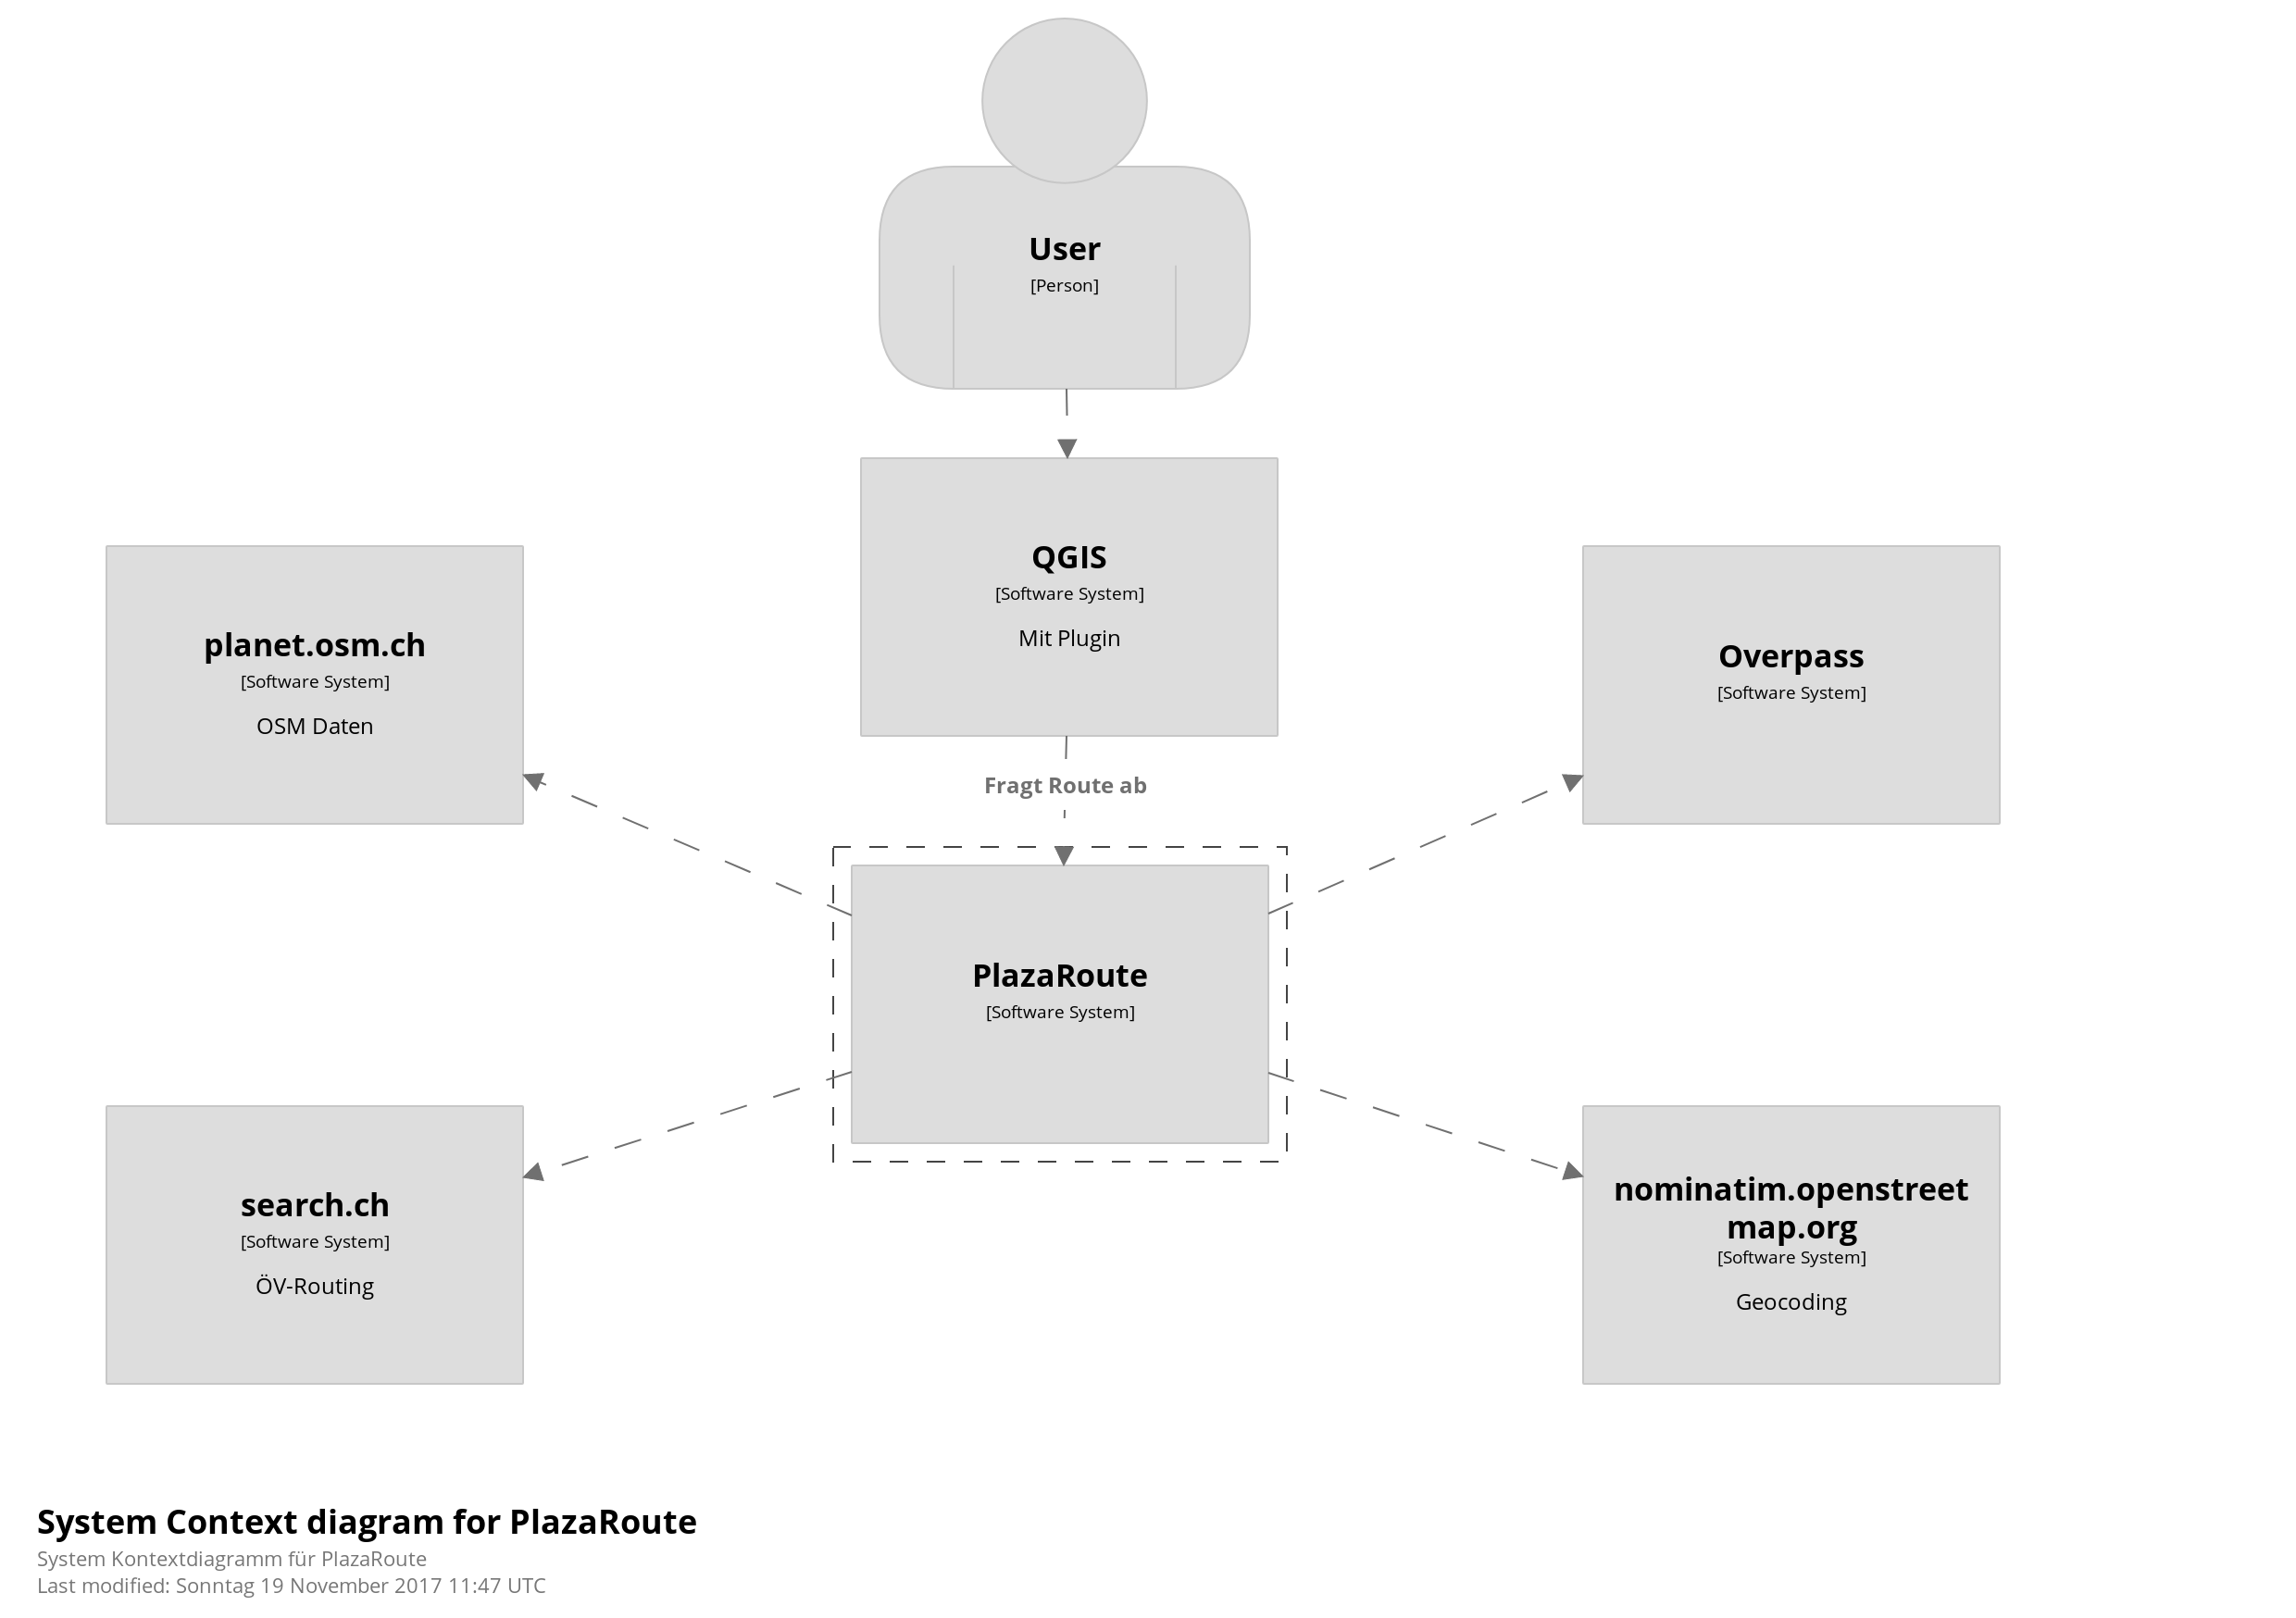
\includegraphics[width=1\linewidth]{projectdoc/img/system-context_diagram.png}
\caption[System Kontext Diagramm]{System PlazaRoute im Kontext mit Umsystemen; Grafik erstellt mit \emph{Structurizr Express}\cite{structurizr}}
\label{fig:system_context_diagram}
\end{figure}

Abbildung \ref{fig:system_context_diagram} zeigt das System PlazaRoute mit den Umsystemen auf.

Der User bedient die QGIS Desktop Applikation mit dem von uns entwickelten Plugin. Dieses leitet die die Eingabe der Start- und Zielkoordinaten an das System PlazaRoute weiter. Als Antwort sendet PlazaRoute eine Routenbeschreibung an das QGIS-Plugin zurück, das es im QGIS darstellt.

\subsection{QGIS Plugin}
\label{architektur:QGIS Plugin}
Das QGIS-Plugin ist unabhängig vom System PlazaRoute und läuft auf dem Client des Benutzers. Die Kommunikation mit dem Container Plaza Routing erfolgt mit HTTPS.
% TODO: Mehr Detail, sobald wir mehr wissen

\subsection{PlazaRoute Container}
\label{architektur:PlazaRoute Container}

\begin{figure}[ht]
    \centering
    % TODO: Grafik zuschneiden
    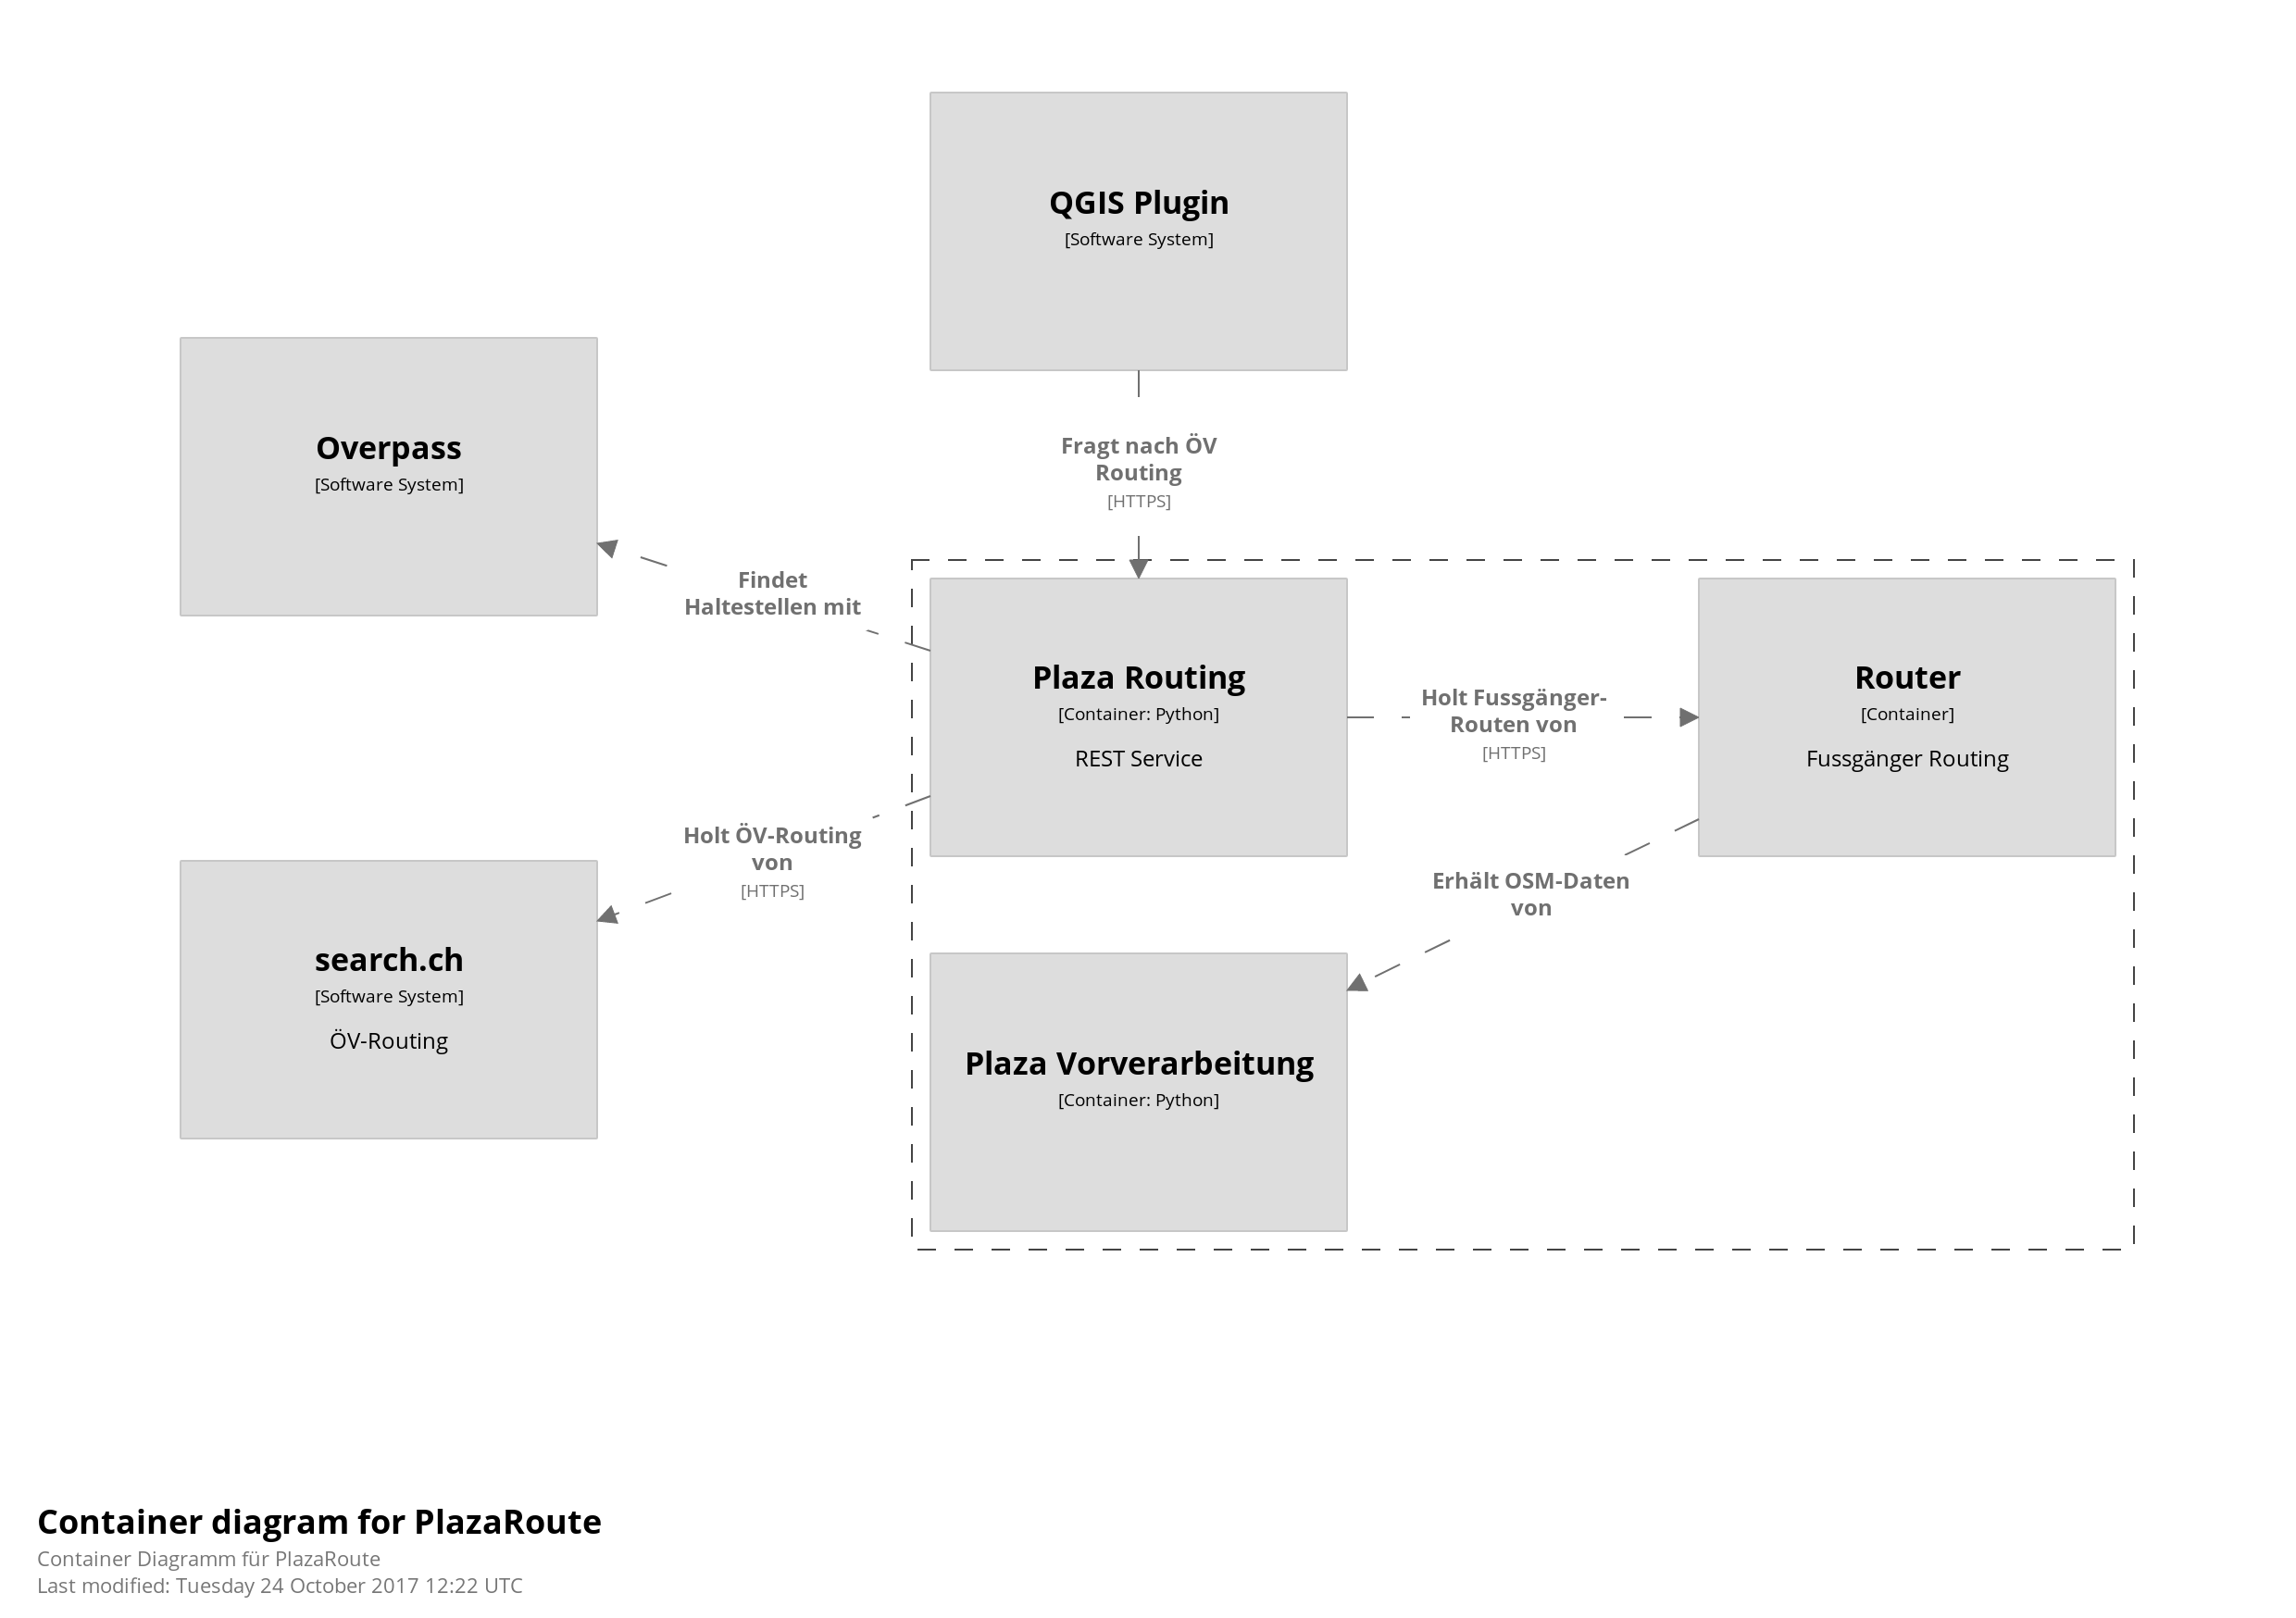
\includegraphics[width=1\linewidth]{projectdoc/img/container_diagram.png}
    \caption[Container Diagramm]{Container Diagramm von PlazaRoute; Grafik erstellt mit \emph{Structurizr Express}\cite{structurizr}}
    \label{fig:container_diagram}
    \end{figure}    

In Abbildung \ref{fig:container_diagram} zoomen wir in das System PlazaRoute hinein und teilen es in drei Container auf, die logisch voneinander getrennt sind. So könnten die Container auch verteilt deployed werden.

In den nachfolgenden Abschnitten werden die drei Container näher beleuchtet.


\subsubsection{Plaza Vorverarbeitung}
\label{architektur:Plaza Vorverarbeitung}

Bevor die Routing Engine ihre Routing-Funktion ausführen kann, muss diese zuerst aus dem \ac{OSM}-Datensatz einen Routing-Graph generieren. Unsere Hauptaufgabe besteht darin, diesen Routing-Graphen für Fussgänger-Routing über Flächen zu optimieren. Ein Ansatz wäre, den Graphen nach dem Generieren zu verändern. Dies ist aber schwer realisierbar, da die meisten Routing-Engines die Graphen in eigenen (binären) Datenstrukturen ablegen. So wär unsere Implementation auch stark an eine einzelne Routing-Engine gekoppelt.

Ein zweiter Ansatz die Integration unserer Optimierung in die Verarbeitung der Routing-Engines selbst. Auch da wären wir wieder stark an eine spezifische Routing-Engine gekoppelt.
Wir haben uns stattdessen entschieden, beim Input der \ac{OSM}-Daten anzusetzen. Dazu werden die Rohdaten zuerst eingelesen und nach Fussgänger-Flächen abgesucht (\nameref{par:OSM Importer}). Mit unserem Algorithmus werden neue Fusswege eingetragen (\nameref{par:Plaza Optimizer}). Diese neu erzeugten Kartendaten werden dann wieder mit den ursprünglichen Rohdaten verschmelzt (\nameref{par:OSM Merger}). Erst dann generiert die Routing-Engine daraus den Routing-Graphen. Das Vorgehen ist in Abbildung \ref{fig:workflow_vorverarbeitung} schematisch aufgezeigt.

Abbildung \ref{fig:component_diagram_vorverarbeitung} zeigt die einzelnen Komponenten für die Vorverarbeitung der \ac{OSM}-Daten auf.


\begin{figure}[ht]
    \centering
    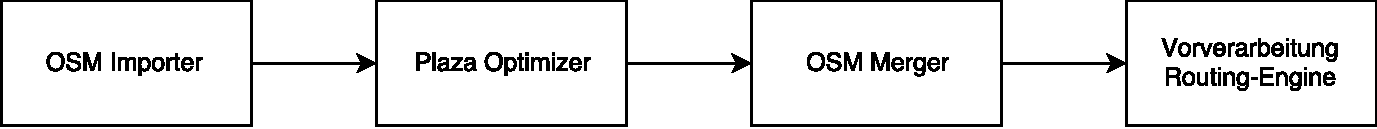
\includegraphics[width=1\linewidth]{projectdoc/img/workflow_vorverarbeitung.pdf}
    \caption[Ablauf Vorverarbeitung]{Ablauf der Vorverarbeitung der \ac{OSM}-Daten bis zur Übergabe an die Routing-Engine; Grafik erstellt mit \emph{draw.io}}
    \label{fig:workflow_vorverarbeitung}
\end{figure}
    

\begin{figure}[ht]
\centering
% TODO: Grafik zuschneiden
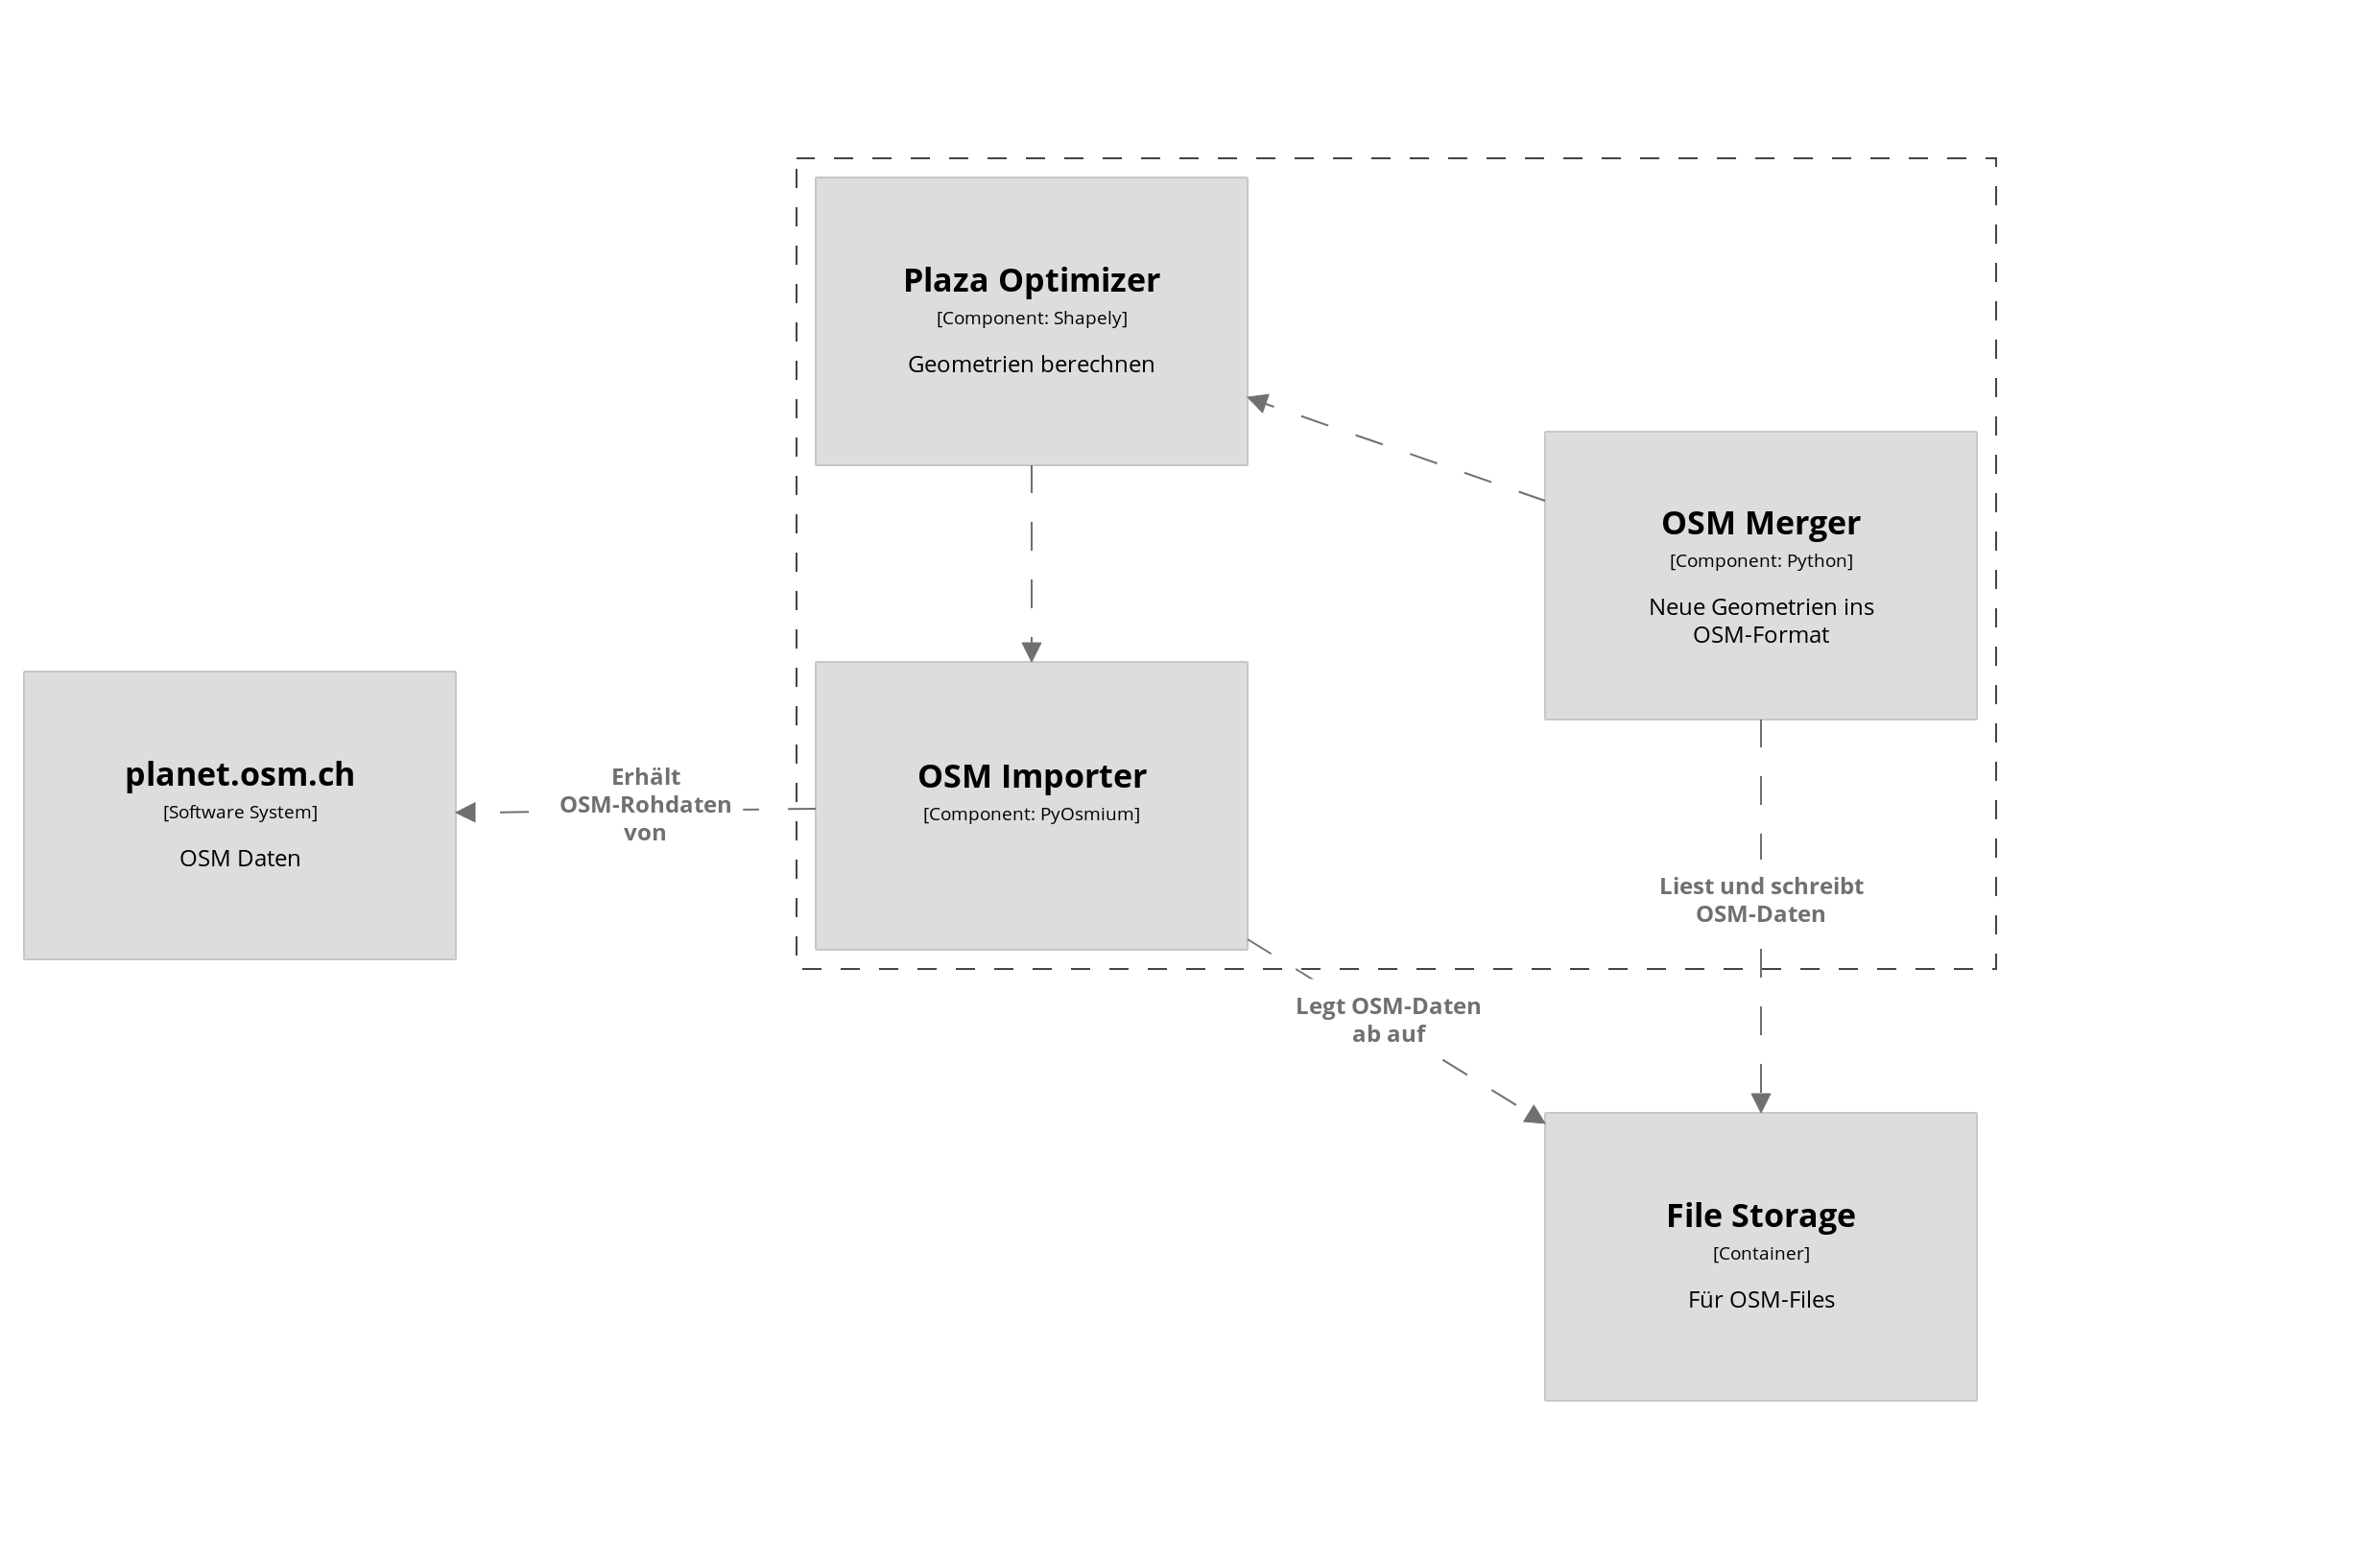
\includegraphics[width=1\linewidth]{projectdoc/img/component_diagram_plaza-vorverarbeitung.png}
\caption[Komponentendiagramm Vorverarbeitung]{Komponentendiagramm der Plaza Vorverarbeitung; Grafik erstellt mit \emph{Structurizr Express}\cite{structurizr}}
\label{fig:component_diagram_vorverarbeitung}
\end{figure}


\paragraph{OSM Importer}\label{par:OSM Importer}~\\
Für unser optimiertes Routing wird in regelmässigen Abständen der neueste \ac{OSM}-Datensatz \cite{osm_data_switzerland} der Schweiz geladen. Die \acs{OSM}-Importer Komponente liest das komplette für uns relevante Kartenmaterial (z.B. die Schweiz) als \ac{PBF} ein und sucht dabei nach Flächen, die wir bearbeiten wollen.

Dazu werden \emph{Osmium} und die dazugehörigen Python-Bindings \emph{pyOsmium}\cite{pyosmium} verwendet. Osmium erkennt automatisch Flächen aus \ac{OSM} Multipolygone oder Relationen. Mit einem eigenen Handler können wir dabei gleich das Einlesen des Files auf die für uns interessanten Flächen beschränken, wie in Listing \ref{osmium_import_code} gezeigt wird.

%TODO: In Implementation verschieben?

\begin{listing}[ht]
    \inputminted{python}{projectdoc/listing/osmium_handler.py}
    \caption[Einlesen OSM-Daten mit Osmium]{Einlesen von OSM Daten mithilfe von \emph{Osmium}; Filterung auf für uns relevante Flächen}
    \label{osmium_import_code}
\end{listing}

\paragraph{Plaza Optimizer}\label{par:Plaza Optimizer}~\\
Die mit Osmium importierten \ac{OSM}-Daten sind noch reine \ac{OSM}-Objekte, auf denen keine Geometrie-Berechnungen angewendet werden können. Dazu wird die Python-Library \emph{Shapely}\cite{shapely} verwendet. Shapely kann mit Geometrien umgehen und Algorithmen von \ac{GEOS} wie \code{intersection} und \code{contains} darauf anwenden.

Um die mit Osmium importierten Objekte in Shapely zu verwenden, werden diese ins \ac{WKB} Format übersetzt und Shapely übergeben, wie in Listing \ref{shapely_import_code} gezeigt.

\begin{listing}[ht]
    \inputminted{python}{projectdoc/listing/shapely_import.py}
    \caption[Einlesen OSM Objekte in Shapely]{Übergabe von Osmium-Objekten zu Shapely für die Weiterverarbeitung}
    \label{shapely_import_code}
\end{listing}



\paragraph{OSM Merger}\label{par:OSM Merger}~\\
Der OSM Merger ist dafür verantwortlich, unsere erzeugten Geometrien (Fusswege) wieder in das \ac{OSM}-Kartenmaterial einzupflegen, um es anschliessend der Routing-Engine zur Verarbeitung zum Routing-Graphen zu übergeben.

Die durch unseren Algorithmus erzeugten Wege durch Flächen (in Shapely Datenstrukturen) sollen nun wieder zurück ins \ac{OSM}-Format geschrieben werden. Dazu wird wie beim \nameref{par:OSM Importer} Osmium verwendet, mit dem Geometrien in eine OSM-Datei geschrieben werden können

In einem weiteren Schritt müssen unsere optimierten Wege in das bestehende Strassennetz eingebunden werden, damit die Routing-Engine diese auch beachtet. Dazu werden die Eingangspunkte der von uns erzeugten Fusswege in den bestehenden Strassen und Wegen referenziert, die an diesem Punkt auf die Fläche treffen. Somit werden sie topologisch direkt miteinander verbunden.
% TODO: Begriff Eintrittspunkt definieren

Als letzten Schritt führen wir die erzeugten Fusswege und die modifizierten Strassen wieder zusammen mit der "grossen" \ac{OSM}-Datei, die ganz am Anfang importiert wurde. Dazu wird das Commandline-Tool Osmosis \cite{osmosis} verwendet.

\subsubsection{Plaza Routing}
\label{architektur:Plaza Routing}
Der Plaza Routing Container (siehe Abbildung \ref{fig:container_diagram}) ist für das Koordinieren und Verabeiten von Routing-Anfragen verantwortlich. Er bietet für das QGIS-Plugin eine API an. Mit Hilfe von search.ch (für ÖV-Routing) und der Routing-Engine (für Fussgänger-Routing) wird eine komplette Route mit Fahrplan erstellt und dem QGIS-Plugin übergeben.

\paragraph{Schnittstelle}\label{architektur:Schnittstelle}~\\
%TODO Interface, welches nach aussen exponiert wird mit Swagger
TODO

\paragraph{Routing-Engine Anbindung}\label{architektur:Routing-Engine Anbindung}~\\
%TODO Strategy-Pattern beschreiben, welches verwendet wird, damit Routing-Engine ausgetauscht werden kann
TODO


\paragraph{Overpass Anbindung}\label{architektur:Overpass Anbindung}~\\
TODO

\paragraph{Search.ch Anbindung}\label{architektur:Search.ch Anbindung}~\\
TODO



